\begin{figure*}
\centering
\begin{subfigure}[b]{.24\textwidth}
%\includegraphics[width=\textwidth]{input_space}
\begin{tikzpicture}[scale=.5,y=-0.80pt, x=0.8pt]
\begin{scope}
\begin{scope}% layer1
    \draw[fill=gray, draw=black,  line width=2]  (142,195) node (a) {} circle (6pt);
    \draw[fill=gray, draw=black,  line width=2]  (95,202) node (b) {} circle (6pt); 
    \draw[fill=gray, draw=black,  line width=2]  (122,155) node (c) {} circle (6pt);  
    \draw[fill=gray, draw=black,  line width=2]  (160,152) node (d) {} circle (6pt);  
     \draw[fill=gray, draw=black,  line width=2]  (170,225)node (e) {}  circle (6pt);  
      \draw[fill=gray, draw=black,  line width=2]  (185,185) node (f) {} circle (6pt);  
      \begin{pgfonlayer}{quadcell}
     \filldraw[color=gray]  (b.center) -- (c.center) -- (d.center) -- (f.center) --  (e.center) -- cycle;
     \end{pgfonlayer}
      \begin{pgfonlayer}{edges}
      \path[color=black, line width=2] (a.center) edge (b.center);
      \path[color=black, line width=2] (a.center) edge (c.center);
      \path[color=black, line width=2] (a.center) edge (d.center);
      \path[color=black, line width=2] (a.center) edge (e.center);
      \path[color=black, line width=2] (a.center) edge (f.center);
      \path[color=black, line width=2] (e.center) edge (f.center) edge (b.center);
      \path[color=black, line width=2] (c.center) edge (b.center) edge (d.center);
       \path[color=black, line width=2] (d.center) edge (f.center);
       \path[color=black, line width =2] (122,155) edge (80, 90);
      \end{pgfonlayer}
\end{scope}
    \begin{scope}[shift={(125,284)},rotate=120]
    \draw[fill=gray, draw=black,  line width=2]  (142,195) node (a) {} circle (6pt);
    \draw[fill=gray, draw=black,  line width=2]  (95,202) node (b) {} circle (6pt); 
    \draw[fill=gray, draw=black,  line width=2]  (122,155) node (c) {} circle (6pt);  
    \draw[fill=gray, draw=black,  line width=2]  (160,152) node (d) {} circle (6pt);  
     \draw[fill=gray, draw=black,  line width=2]  (170,225)node (e) {}  circle (6pt);  
      \draw[fill=gray, draw=black,  line width=2]  (185,185) node (f) {} circle (6pt);  
      \begin{pgfonlayer}{quadcell}
     \filldraw[color=gray]  (b.center) -- (c.center) -- (d.center) -- (f.center) --  (e.center) -- cycle;
     \end{pgfonlayer}
      \begin{pgfonlayer}{edges}
      \path[color=black, line width=2] (a.center) edge (b.center);
      \path[color=black, line width=2] (a.center) edge (c.center);
      \path[color=black, line width=2] (a.center) edge (d.center);
      \path[color=black, line width=2] (a.center) edge (e.center);
      \path[color=black, line width=2] (a.center) edge (f.center);
      \path[color=black, line width=2] (e.center) edge (f.center) edge (b.center);
      \path[color=black, line width=2] (c.center) edge (b.center) edge (d.center);
       \path[color=black, line width=2] (d.center) edge (f.center);
          \path[color=black, line width =2] (160, 152) edge (200, 90);
      \end{pgfonlayer}
                \end{scope}
        \begin{scope}[shift={(198,-138)},rotate=-70]
    \draw[fill=gray, draw=black,  line width=2]  (142,195) node (a) {} circle (6pt);
    \draw[fill=gray, draw=black,  line width=2]  (95,202) node (b) {} circle (6pt); 
    \draw[fill=gray, draw=black,  line width=2]  (122,155) node (c) {} circle (6pt);  
    \draw[fill=gray, draw=black,  line width=2]  (160,152) node (d) {} circle (6pt);  
     \draw[fill=gray, draw=black,  line width=2]  (170,225)node (e) {}  circle (6pt);  
      \draw[fill=gray, draw=black,  line width=2]  (185,185) node (f) {} circle (6pt);  
      \begin{pgfonlayer}{quadcell}
     \filldraw[color=gray]  (b.center) -- (c.center) -- (d.center) -- (f.center) --  (e.center) -- cycle;
     \end{pgfonlayer}
           \begin{pgfonlayer}{edges}
      \path[color=black, line width=2] (a.center) edge (b.center);
      \path[color=black, line width=2] (a.center) edge (c.center);
      \path[color=black, line width=2] (a.center) edge (d.center);
      \path[color=black, line width=2] (a.center) edge (e.center);
      \path[color=black, line width=2] (a.center) edge (f.center);
      \path[color=black, line width=2] (e.center) edge (f.center) edge (b.center);
      \path[color=black, line width=2] (c.center) edge (b.center) edge (d.center);
       \path[color=black, line width=2] (d.center) edge (f.center);
      \end{pgfonlayer}
         \end{scope}
  \end{scope}
\end{tikzpicture}
\caption{Input Complex $\K$}
\label{fig:input}
\end{subfigure}
\hfill
\begin{subfigure}[b]{.24\textwidth}
\begin{tikzpicture}[scale=.5,y=-0.80pt, x=0.8pt]
\begin{scope}% layer1
    \draw[fill=afrapurple, draw=black,  line width=1]  (142,195) node (a) {} circle (6pt);
    \draw[fill=afrapurple, draw=black,  line width=1]  (95,202) node (b) {} circle (6pt); 
    \draw[fill=afrapurple, draw=black,  line width=1]  (122,155) node (c) {} circle (6pt);  
    \draw[fill=afrapurple, draw=black,  line width=1]  (160,152) node (d) {} circle (6pt);  
     \draw[fill=afrapurple, draw=black,  line width=1]  (170,225)node (e) {}  circle (6pt);  
      \draw[fill=afrapurple, draw=black,  line width=1]  (185,185) node (f) {} circle (6pt);  
    \begin{scope}% g10596
      % path7778
      \path[draw=afrapurplelight,line join=miter,line cap=butt,miter limit=4.00,line
        width=2] (142.8068,141.8195) .. controls (140.5229,140.7866) and
        (138.2447,139.7410) .. (135.9724,138.6829) .. controls (133.0686,137.3306) and
        (130.1306,135.9436) .. (126.9750,135.3928) .. controls (123.2061,134.7350) and
        (119.2405,135.3312) .. (115.7977,137.0000) .. controls (112.3550,138.6687) and
        (109.4446,141.3929) .. (107.4859,144.6794) .. controls (105.5194,147.9789) and
        (104.5226,151.7563) .. (103.6919,155.5065) .. controls (102.8612,159.2568) and
        (102.1647,163.0652) .. (100.7192,166.6240) .. controls (98.5492,171.9661) and
        (94.7943,176.4976) .. (90.9055,180.7549) .. controls (87.1005,184.9204) and
        (83.0614,188.9825) .. (80.3662,193.9388) .. controls (79.0186,196.4170) and
        (78.0238,199.1093) .. (77.6619,201.9068) .. controls (77.2999,204.7044) and
        (77.5891,207.6123) .. (78.7040,210.2036) .. controls (79.9202,213.0305) and
        (82.0576,215.3721) .. (84.4182,217.3464) .. controls (89.4627,221.5653) and
        (95.5940,224.2926) .. (101.8472,226.3281) .. controls (108.1004,228.3635) and
        (114.5437,229.7569) .. (120.8468,231.6321) .. controls (125.8989,233.1351) and
        (130.8532,234.9453) .. (135.8468,236.6321) .. controls (143.5496,239.2340) and
        (151.4656,241.5630) .. (159.5933,241.7724) .. controls (167.7210,241.9818) and
        (176.1768,239.8661) .. (182.2754,234.4893) .. controls (186.9397,230.3769) and
        (189.9191,224.6670) .. (192.0037,218.8085) .. controls (194.0883,212.9500) and
        (195.3761,206.8390) .. (197.2754,200.9178) .. controls (198.3603,197.5357) and
        (199.6460,194.2112) .. (200.4716,190.7566) .. controls (201.2972,187.3020) and
        (201.6504,183.6634) .. (200.8468,180.2036) .. controls (200.0756,176.8833) and
        (198.2661,173.8691) .. (196.0175,171.3074) .. controls (193.7689,168.7456) and
        (191.0857,166.6035) .. (188.3386,164.5855) .. controls (182.8445,160.5494) and
        (176.8474,156.7588) .. (173.3140,150.9287) .. controls (171.6874,148.2446) and
        (170.6556,145.2291) .. (168.9715,142.5808) .. controls (168.1294,141.2566) and
        (167.1180,140.0232) .. (165.8705,139.0712) .. controls (164.6230,138.1193) and
        (163.1264,137.4584) .. (161.5611,137.3464) .. controls (160.3978,137.2632) and
        (159.2270,137.4826) .. (158.1251,137.8650) .. controls (157.0233,138.2474) and
        (155.9841,138.7900) .. (154.9709,139.3678) .. controls (152.9447,140.5234) and
        (150.9545,141.8488) .. (148.6798,142.3654) .. controls (146.7303,142.8081) and
        (144.6414,142.6140) .. (142.8068,141.8195);
    \end{scope}
        
    \begin{scope}[shift={(125,284)},rotate=120]
    \draw[fill=afragreen,draw=black,  line width=1]  (142,195) node (a) {} circle (6pt);
    \draw[fill=afragreen, draw=black,  line width=1]  (95,202) node (b) {} circle (6pt); 
    \draw[fill=afragreen, draw=black,  line width=1]  (122,155) node (c) {} circle (6pt);  
    \draw[fill=afragreen, draw=black,  line width=1]  (160,152) node (d) {} circle (6pt);  
     \draw[fill=afragreen, draw=black,  line width=1]  (170,225)node (e) {}  circle (6pt);  
      \draw[fill=afragreen, draw=black,  line width=1]  (185,185) node (f) {} circle (6pt);  
                \end{scope}
    \begin{scope}% g10596
      % path7778
            % path7778-9
      \path[draw=afragreenlight,line join=miter,line cap=butt,miter limit=4.00,line
        width=2] (192.9926,11.9341) .. controls (188.8896,12.6152) and
        (184.9965,14.4282) .. (181.7524,17.0311) .. controls (178.5084,19.6340) and
        (175.9104,23.0138) .. (174.1113,26.7637) .. controls (169.8923,35.5570) and
        (170.1687,45.8307) .. (167.1178,55.0943) .. controls (165.7925,59.1182) and
        (163.8223,63.0319) .. (163.6387,67.2645) .. controls (163.5263,69.8555) and
        (164.1014,72.4453) .. (165.0598,74.8551) .. controls (166.0182,77.2650) and
        (167.3530,79.5081) .. (168.7982,81.6615) .. controls (171.6886,85.9684) and
        (175.0752,90.0199) .. (177.0385,94.8209) .. controls (177.8932,96.9111) and
        (178.4609,99.1056) .. (179.1934,101.2417) .. controls (179.9259,103.3778) and
        (180.8444,105.4903) .. (182.2959,107.2203) .. controls (183.6446,108.8277) and
        (185.4163,110.0510) .. (187.3327,110.9055) .. controls (189.2491,111.7601) and
        (191.3102,112.2567) .. (193.3884,112.5466) .. controls (197.5448,113.1264) and
        (201.7732,112.8927) .. (205.9513,113.2866) .. controls (211.2015,113.7817) and
        (216.3028,115.2594) .. (221.4846,116.2387) .. controls (229.3108,117.7177) and
        (237.3906,118.0536) .. (245.2523,116.7765) .. controls (253.1139,115.4994) and
        (260.7551,112.5790) .. (267.2111,107.9146) .. controls (272.7152,103.9381) and
        (277.3945,98.5796) .. (279.6336,92.1691) .. controls (280.7532,88.9639) and
        (281.2461,85.5266) .. (280.9380,82.1454) .. controls (280.6298,78.7643) and
        (279.5090,75.4439) .. (277.5935,72.6407) .. controls (274.9928,68.8349) and
        (271.0961,66.1511) .. (267.3573,63.4550) .. controls (263.6185,60.7588) and
        (259.8383,57.8362) .. (257.6523,53.7779) .. controls (255.1375,49.1092) and
        (255.0539,43.5530) .. (255.1757,38.2515) .. controls (255.2975,32.9500) and
        (255.5337,27.4624) .. (253.5453,22.5464) .. controls (252.0356,18.8141) and
        (249.2746,15.6239) .. (245.8724,13.4712) .. controls (242.4702,11.3185) and
        (238.4491,10.1936) .. (234.4237,10.1225) .. controls (228.1091,10.0111) and
        (222.0000,12.4065) .. (215.6949,12.7688) .. controls (208.1147,13.2044) and
        (200.4828,10.6908) .. (192.9926,11.9341);
    \end{scope}
        \begin{scope}[shift={(198,-138)},rotate=-70]
    \draw[fill=afrablue, draw=black,  line width=1]  (142,195) node (a) {} circle (6pt);
    \draw[fill=afrablue,draw=black,  line width=1]  (95,202) node (b) {} circle (6pt); 
    \draw[fill=afrablue, draw=black,  line width=1]  (122,155) node (c) {} circle (6pt);  
    \draw[fill=afrablue, draw=black,  line width=1]  (160,152) node (d) {} circle (6pt);  
     \draw[fill=afrablue, draw=black,  line width=1]  (170,225)node (e) {}  circle (6pt);  
      \draw[fill=afrablue, draw=black,  line width=1]  (185,185) node (f) {} circle (6pt);  
         \end{scope}
    \begin{scope}% g10596
      % path7778-4
      \path[draw=afrabluedark,line join=miter,line cap=butt,miter limit=4.00,line
        width=2] (114.2167,41.2393) .. controls (111.5795,35.7883) and
        (110.3171,29.7694) .. (107.8770,24.2274) .. controls (106.6569,21.4563) and
        (105.1297,18.7930) .. (103.0913,16.5543) .. controls (101.0528,14.3156) and
        (98.4767,12.5121) .. (95.5673,11.6741) .. controls (93.1997,10.9921) and
        (90.6823,10.9636) .. (88.2376,11.2700) .. controls (85.7928,11.5764) and
        (83.4024,12.2091) .. (81.0192,12.8346) .. controls (78.6361,13.4602) and
        (76.2421,14.0821) .. (73.7946,14.3663) .. controls (71.3472,14.6505) and
        (68.8282,14.5876) .. (66.4734,13.8627) .. controls (64.2730,13.1855) and
        (62.2883,11.9568) .. (60.3633,10.6941) .. controls (58.4383,9.4313) and
        (56.5283,8.1123) .. (54.4053,7.2216) .. controls (51.6098,6.0489) and
        (48.5082,5.6617) .. (45.4923,5.9694) .. controls (42.4764,6.2771) and
        (39.5466,7.2678) .. (36.8902,8.7284) .. controls (31.5772,11.6495) and
        (27.4415,16.3672) .. (24.2232,21.5057) .. controls (22.6382,24.0364) and
        (21.2430,26.7025) .. (20.3036,29.5370) .. controls (18.2838,35.6312) and
        (18.4521,42.2521) .. (19.4464,48.5949) .. controls (20.4406,54.9377) and
        (22.2309,61.1289) .. (23.4110,67.4398) .. controls (24.3531,72.4776) and
        (24.9041,77.5791) .. (25.4838,82.6714) .. controls (26.3970,90.6930) and
        (27.4212,98.8460) .. (30.7141,106.2174) .. controls (32.3605,109.9031) and
        (34.5756,113.3615) .. (37.4426,116.2032) .. controls (40.3097,119.0448) and
        (43.8461,121.2553) .. (47.7398,122.3203) .. controls (53.5513,123.9098) and
        (59.7541,122.8914) .. (65.5662,121.3043) .. controls (71.3782,119.7172) and
        (77.0782,117.5626) .. (83.0613,116.8547) .. controls (86.5271,116.4447) and
        (90.0380,116.5279) .. (93.5015,116.0988) .. controls (96.9650,115.6697) and
        (100.4817,114.6656) .. (103.1342,112.3975) .. controls (104.6594,111.0933) and
        (105.8396,109.4167) .. (106.7141,107.6106) .. controls (107.5886,105.8044) and
        (108.1667,103.8674) .. (108.6010,101.9082) .. controls (109.4697,97.9899) and
        (109.7788,93.9469) .. (110.9329,90.1030) .. controls (112.5367,84.7609) and
        (115.6923,80.0478) .. (118.3166,75.1262) .. controls (119.6288,72.6653) and
        (120.8193,70.1251) .. (121.6073,67.4499) .. controls (122.3953,64.7747) and
        (122.7732,61.9521) .. (122.4431,59.1829) .. controls (122.0511,55.8942) and
        (120.6821,52.7996) .. (119.0883,49.8963) .. controls (117.4945,46.9930) and
        (115.6592,44.2207) .. (114.2167,41.2393);
    \end{scope}
  \end{scope}
\end{tikzpicture}
\caption{Partition $P$}
\label{fig:part}
\end{subfigure}
\hfill
\begin{subfigure}[b]{.24\textwidth}
\begin{tikzpicture}[scale=.5,y=-0.80pt, x=0.8pt]
\begin{scope}

\begin{scope}% layer1
    \draw[fill=afrapurple, draw=afrapurpledark,  line width=2]  (142,195) node (a) {} circle (6pt);
    \draw[fill=afrapurple, draw=afrapurpledark,  line width=2]  (95,202) node (b) {} circle (6pt); 
    \draw[fill=afrapurple, draw=afrapurpledark,  line width=2]  (122,155) node (c) {} circle (6pt);  
    \draw[fill=afrapurple, draw=afrapurpledark,  line width=2]  (160,152) node (d) {} circle (6pt);  
     \draw[fill=afrapurple, draw=afrapurpledark,  line width=2]  (170,225)node (e) {}  circle (6pt);  
      \draw[fill=afrapurple, draw=afrapurpledark,  line width=2]  (185,185) node (f) {} circle (6pt);  
      \begin{pgfonlayer}{quadcell}
     \filldraw[color=afrapurple]  (b.center) -- (c.center) -- (d.center) -- (f.center) --  (e.center) -- cycle;
     \end{pgfonlayer}
      \begin{pgfonlayer}{edges}
      \path[color=afrapurpledark, line width=2] (a.center) edge (b.center);
      \path[color=afrapurpledark, line width=2] (a.center) edge (c.center);
      \path[color=afrapurpledark, line width=2] (a.center) edge (d.center);
      \path[color=afrapurpledark, line width=2] (a.center) edge (e.center);
      \path[color=afrapurpledark, line width=2] (a.center) edge (f.center);
      \path[color=afrapurpledark, line width=2] (e.center) edge (f.center) edge (b.center);
      \path[color=afrapurpledark, line width=2] (c.center) edge (b.center) edge (d.center);
       \path[color=afrapurpledark, line width=2] (d.center) edge (f.center);
       \path[color=gray, line width =2] (122,155) edge (80, 90);
      \end{pgfonlayer}
    \begin{scope}% g10596
      % path7778
      \path[draw=afrapurplelight,line join=miter,line cap=butt,miter limit=4.00,line
        width=2] (142.8068,141.8195) .. controls (140.5229,140.7866) and
        (138.2447,139.7410) .. (135.9724,138.6829) .. controls (133.0686,137.3306) and
        (130.1306,135.9436) .. (126.9750,135.3928) .. controls (123.2061,134.7350) and
        (119.2405,135.3312) .. (115.7977,137.0000) .. controls (112.3550,138.6687) and
        (109.4446,141.3929) .. (107.4859,144.6794) .. controls (105.5194,147.9789) and
        (104.5226,151.7563) .. (103.6919,155.5065) .. controls (102.8612,159.2568) and
        (102.1647,163.0652) .. (100.7192,166.6240) .. controls (98.5492,171.9661) and
        (94.7943,176.4976) .. (90.9055,180.7549) .. controls (87.1005,184.9204) and
        (83.0614,188.9825) .. (80.3662,193.9388) .. controls (79.0186,196.4170) and
        (78.0238,199.1093) .. (77.6619,201.9068) .. controls (77.2999,204.7044) and
        (77.5891,207.6123) .. (78.7040,210.2036) .. controls (79.9202,213.0305) and
        (82.0576,215.3721) .. (84.4182,217.3464) .. controls (89.4627,221.5653) and
        (95.5940,224.2926) .. (101.8472,226.3281) .. controls (108.1004,228.3635) and
        (114.5437,229.7569) .. (120.8468,231.6321) .. controls (125.8989,233.1351) and
        (130.8532,234.9453) .. (135.8468,236.6321) .. controls (143.5496,239.2340) and
        (151.4656,241.5630) .. (159.5933,241.7724) .. controls (167.7210,241.9818) and
        (176.1768,239.8661) .. (182.2754,234.4893) .. controls (186.9397,230.3769) and
        (189.9191,224.6670) .. (192.0037,218.8085) .. controls (194.0883,212.9500) and
        (195.3761,206.8390) .. (197.2754,200.9178) .. controls (198.3603,197.5357) and
        (199.6460,194.2112) .. (200.4716,190.7566) .. controls (201.2972,187.3020) and
        (201.6504,183.6634) .. (200.8468,180.2036) .. controls (200.0756,176.8833) and
        (198.2661,173.8691) .. (196.0175,171.3074) .. controls (193.7689,168.7456) and
        (191.0857,166.6035) .. (188.3386,164.5855) .. controls (182.8445,160.5494) and
        (176.8474,156.7588) .. (173.3140,150.9287) .. controls (171.6874,148.2446) and
        (170.6556,145.2291) .. (168.9715,142.5808) .. controls (168.1294,141.2566) and
        (167.1180,140.0232) .. (165.8705,139.0712) .. controls (164.6230,138.1193) and
        (163.1264,137.4584) .. (161.5611,137.3464) .. controls (160.3978,137.2632) and
        (159.2270,137.4826) .. (158.1251,137.8650) .. controls (157.0233,138.2474) and
        (155.9841,138.7900) .. (154.9709,139.3678) .. controls (152.9447,140.5234) and
        (150.9545,141.8488) .. (148.6798,142.3654) .. controls (146.7303,142.8081) and
        (144.6414,142.6140) .. (142.8068,141.8195);
    \end{scope}
        \end{scope}
        
    \begin{scope}[shift={(125,284)},rotate=120]
    \draw[fill=afragreen, draw=afragreendark,  line width=2]  (142,195) node (a) {} circle (6pt);
    \draw[fill=afragreen, draw=afragreendark,  line width=2]  (95,202) node (b) {} circle (6pt); 
    \draw[fill=afragreen, draw=afragreendark,  line width=2]  (122,155) node (c) {} circle (6pt);  
    \draw[fill=afragreen, draw=afragreendark,  line width=2]  (160,152) node (d) {} circle (6pt);  
     \draw[fill=afragreen, draw=afragreendark,  line width=2]  (170,225)node (e) {}  circle (6pt);  
      \draw[fill=afragreen, draw=afragreendark,  line width=2]  (185,185) node (f) {} circle (6pt);  
      \begin{pgfonlayer}{quadcell}
     \filldraw[color=afragreen]  (b.center) -- (c.center) -- (d.center) -- (f.center) --  (e.center) -- cycle;
     \end{pgfonlayer}
      \begin{pgfonlayer}{edges}
      \path[color=afragreendark, line width=2] (a.center) edge (b.center);
      \path[color=afragreendark, line width=2] (a.center) edge (c.center);
      \path[color=afragreendark, line width=2] (a.center) edge (d.center);
      \path[color=afragreendark, line width=2] (a.center) edge (e.center);
      \path[color=afragreendark, line width=2] (a.center) edge (f.center);
      \path[color=afragreendark, line width=2] (e.center) edge (f.center) edge (b.center);
      \path[color=afragreendark, line width=2] (c.center) edge (b.center) edge (d.center);
       \path[color=afragreendark, line width=2] (d.center) edge (f.center);
          \path[color=gray, line width =2] (160, 152) edge (200, 90);
      \end{pgfonlayer}
                \end{scope}
    \begin{scope}% g10596
      % path7778
            % path7778-9
      \path[draw=afragreenlight,line join=miter,line cap=butt,miter limit=4.00,line
        width=2] (192.9926,11.9341) .. controls (188.8896,12.6152) and
        (184.9965,14.4282) .. (181.7524,17.0311) .. controls (178.5084,19.6340) and
        (175.9104,23.0138) .. (174.1113,26.7637) .. controls (169.8923,35.5570) and
        (170.1687,45.8307) .. (167.1178,55.0943) .. controls (165.7925,59.1182) and
        (163.8223,63.0319) .. (163.6387,67.2645) .. controls (163.5263,69.8555) and
        (164.1014,72.4453) .. (165.0598,74.8551) .. controls (166.0182,77.2650) and
        (167.3530,79.5081) .. (168.7982,81.6615) .. controls (171.6886,85.9684) and
        (175.0752,90.0199) .. (177.0385,94.8209) .. controls (177.8932,96.9111) and
        (178.4609,99.1056) .. (179.1934,101.2417) .. controls (179.9259,103.3778) and
        (180.8444,105.4903) .. (182.2959,107.2203) .. controls (183.6446,108.8277) and
        (185.4163,110.0510) .. (187.3327,110.9055) .. controls (189.2491,111.7601) and
        (191.3102,112.2567) .. (193.3884,112.5466) .. controls (197.5448,113.1264) and
        (201.7732,112.8927) .. (205.9513,113.2866) .. controls (211.2015,113.7817) and
        (216.3028,115.2594) .. (221.4846,116.2387) .. controls (229.3108,117.7177) and
        (237.3906,118.0536) .. (245.2523,116.7765) .. controls (253.1139,115.4994) and
        (260.7551,112.5790) .. (267.2111,107.9146) .. controls (272.7152,103.9381) and
        (277.3945,98.5796) .. (279.6336,92.1691) .. controls (280.7532,88.9639) and
        (281.2461,85.5266) .. (280.9380,82.1454) .. controls (280.6298,78.7643) and
        (279.5090,75.4439) .. (277.5935,72.6407) .. controls (274.9928,68.8349) and
        (271.0961,66.1511) .. (267.3573,63.4550) .. controls (263.6185,60.7588) and
        (259.8383,57.8362) .. (257.6523,53.7779) .. controls (255.1375,49.1092) and
        (255.0539,43.5530) .. (255.1757,38.2515) .. controls (255.2975,32.9500) and
        (255.5337,27.4624) .. (253.5453,22.5464) .. controls (252.0356,18.8141) and
        (249.2746,15.6239) .. (245.8724,13.4712) .. controls (242.4702,11.3185) and
        (238.4491,10.1936) .. (234.4237,10.1225) .. controls (228.1091,10.0111) and
        (222.0000,12.4065) .. (215.6949,12.7688) .. controls (208.1147,13.2044) and
        (200.4828,10.6908) .. (192.9926,11.9341);
    \end{scope}
        \begin{scope}[shift={(198,-138)},rotate=-70]
    \draw[fill=afrablue, draw=afrabluedark,  line width=2]  (142,195) node (a) {} circle (6pt);
    \draw[fill=afrablue, draw=afrabluedark,  line width=2]  (95,202) node (b) {} circle (6pt); 
    \draw[fill=afrablue, draw=afrabluedark,  line width=2]  (122,155) node (c) {} circle (6pt);  
    \draw[fill=afrablue, draw=afrabluedark,  line width=2]  (160,152) node (d) {} circle (6pt);  
     \draw[fill=afrablue, draw=afrabluedark,  line width=2]  (170,225)node (e) {}  circle (6pt);  
      \draw[fill=afrablue, draw=afrabluedark,  line width=2]  (185,185) node (f) {} circle (6pt);  
      \begin{pgfonlayer}{quadcell}
     \filldraw[color=afrablue]  (b.center) -- (c.center) -- (d.center) -- (f.center) --  (e.center) -- cycle;
     \end{pgfonlayer}
           \begin{pgfonlayer}{edges}
      \path[color=afrabluedark, line width=2] (a.center) edge (b.center);
      \path[color=afrabluedark, line width=2] (a.center) edge (c.center);
      \path[color=afrabluedark, line width=2] (a.center) edge (d.center);
      \path[color=afrabluedark, line width=2] (a.center) edge (e.center);
      \path[color=afrabluedark, line width=2] (a.center) edge (f.center);
      \path[color=afrabluedark, line width=2] (e.center) edge (f.center) edge (b.center);
      \path[color=afrabluedark, line width=2] (c.center) edge (b.center) edge (d.center);
       \path[color=afrabluedark, line width=2] (d.center) edge (f.center);
      \end{pgfonlayer}
         \end{scope}
    \begin{scope}% g10596
      % path7778-4
      \path[draw=afrabluedark,line join=miter,line cap=butt,miter limit=4.00,line
        width=2] (114.2167,41.2393) .. controls (111.5795,35.7883) and
        (110.3171,29.7694) .. (107.8770,24.2274) .. controls (106.6569,21.4563) and
        (105.1297,18.7930) .. (103.0913,16.5543) .. controls (101.0528,14.3156) and
        (98.4767,12.5121) .. (95.5673,11.6741) .. controls (93.1997,10.9921) and
        (90.6823,10.9636) .. (88.2376,11.2700) .. controls (85.7928,11.5764) and
        (83.4024,12.2091) .. (81.0192,12.8346) .. controls (78.6361,13.4602) and
        (76.2421,14.0821) .. (73.7946,14.3663) .. controls (71.3472,14.6505) and
        (68.8282,14.5876) .. (66.4734,13.8627) .. controls (64.2730,13.1855) and
        (62.2883,11.9568) .. (60.3633,10.6941) .. controls (58.4383,9.4313) and
        (56.5283,8.1123) .. (54.4053,7.2216) .. controls (51.6098,6.0489) and
        (48.5082,5.6617) .. (45.4923,5.9694) .. controls (42.4764,6.2771) and
        (39.5466,7.2678) .. (36.8902,8.7284) .. controls (31.5772,11.6495) and
        (27.4415,16.3672) .. (24.2232,21.5057) .. controls (22.6382,24.0364) and
        (21.2430,26.7025) .. (20.3036,29.5370) .. controls (18.2838,35.6312) and
        (18.4521,42.2521) .. (19.4464,48.5949) .. controls (20.4406,54.9377) and
        (22.2309,61.1289) .. (23.4110,67.4398) .. controls (24.3531,72.4776) and
        (24.9041,77.5791) .. (25.4838,82.6714) .. controls (26.3970,90.6930) and
        (27.4212,98.8460) .. (30.7141,106.2174) .. controls (32.3605,109.9031) and
        (34.5756,113.3615) .. (37.4426,116.2032) .. controls (40.3097,119.0448) and
        (43.8461,121.2553) .. (47.7398,122.3203) .. controls (53.5513,123.9098) and
        (59.7541,122.8914) .. (65.5662,121.3043) .. controls (71.3782,119.7172) and
        (77.0782,117.5626) .. (83.0613,116.8547) .. controls (86.5271,116.4447) and
        (90.0380,116.5279) .. (93.5015,116.0988) .. controls (96.9650,115.6697) and
        (100.4817,114.6656) .. (103.1342,112.3975) .. controls (104.6594,111.0933) and
        (105.8396,109.4167) .. (106.7141,107.6106) .. controls (107.5886,105.8044) and
        (108.1667,103.8674) .. (108.6010,101.9082) .. controls (109.4697,97.9899) and
        (109.7788,93.9469) .. (110.9329,90.1030) .. controls (112.5367,84.7609) and
        (115.6923,80.0478) .. (118.3166,75.1262) .. controls (119.6288,72.6653) and
        (120.8193,70.1251) .. (121.6073,67.4499) .. controls (122.3953,64.7747) and
        (122.7732,61.9521) .. (122.4431,59.1829) .. controls (122.0511,55.8942) and
        (120.6821,52.7996) .. (119.0883,49.8963) .. controls (117.4945,46.9930) and
        (115.6592,44.2207) .. (114.2167,41.2393);
    \end{scope}
  \end{scope}
\end{tikzpicture}
\caption{Open Cover $\tilde{\C}$}
\label{fig:cover}
\end{subfigure}
\hfill
\begin{subfigure}[b]{.24\textwidth}
\begin{tikzpicture}[scale=.5,y=-0.80pt, x=0.8pt]
\begin{scope}

\begin{scope}% layer1
    \draw[fill=afrapurple, draw=afrapurpledark,  line width=2]  (142,195) node (a) {} circle (6pt);
    \draw[fill=afrapurple, draw=afrapurpledark,  line width=2]  (95,202) node (b) {} circle (6pt); 
    \draw[fill=afrapurple, draw=afrapurpledark,  line width=2]  (122,155) node (c) {} circle (6pt);  
    \draw[fill=afrapurple, draw=afrapurpledark,  line width=2]  (160,152) node (d) {} circle (6pt);  
     \draw[fill=afrapurple, draw=afrapurpledark,  line width=2]  (170,225)node (e) {}  circle (6pt);  
      \draw[fill=afrapurple, draw=afrapurpledark,  line width=2]  (185,185) node (f) {} circle (6pt);  
      \begin{pgfonlayer}{quadcell}
     \filldraw[color=afrapurple]  (b.center) -- (c.center) -- (d.center) -- (f.center) --  (e.center) -- cycle;
     \end{pgfonlayer}
      \begin{pgfonlayer}{edges}
      \path[color=afrapurpledark, line width=2] (a.center) edge (b.center);
      \path[color=afrapurpledark, line width=2] (a.center) edge (c.center);
      \path[color=afrapurpledark, line width=2] (a.center) edge (d.center);
      \path[color=afrapurpledark, line width=2] (a.center) edge (e.center);
      \path[color=afrapurpledark, line width=2] (a.center) edge (f.center);
      \path[color=afrapurpledark, line width=2] (e.center) edge (f.center) edge (b.center);
      \path[color=afrapurpledark, line width=2] (c.center) edge (b.center) edge (d.center);
       \path[color=afrapurpledark, line width=2] (d.center) edge (f.center);
       \path[color=gray, line width =2] (122,155) edge (80, 90);
      \end{pgfonlayer}
    \begin{scope}% g10596
      % path7778
      \path[draw=afrapurplelight,line join=miter,line cap=butt,miter limit=4.00,line
        width=2] (142.8068,141.8195) .. controls (140.5229,140.7866) and
        (138.2447,139.7410) .. (135.9724,138.6829) .. controls (133.0686,137.3306) and
        (130.1306,135.9436) .. (126.9750,135.3928) .. controls (123.2061,134.7350) and
        (119.2405,135.3312) .. (115.7977,137.0000) .. controls (112.3550,138.6687) and
        (109.4446,141.3929) .. (107.4859,144.6794) .. controls (105.5194,147.9789) and
        (104.5226,151.7563) .. (103.6919,155.5065) .. controls (102.8612,159.2568) and
        (102.1647,163.0652) .. (100.7192,166.6240) .. controls (98.5492,171.9661) and
        (94.7943,176.4976) .. (90.9055,180.7549) .. controls (87.1005,184.9204) and
        (83.0614,188.9825) .. (80.3662,193.9388) .. controls (79.0186,196.4170) and
        (78.0238,199.1093) .. (77.6619,201.9068) .. controls (77.2999,204.7044) and
        (77.5891,207.6123) .. (78.7040,210.2036) .. controls (79.9202,213.0305) and
        (82.0576,215.3721) .. (84.4182,217.3464) .. controls (89.4627,221.5653) and
        (95.5940,224.2926) .. (101.8472,226.3281) .. controls (108.1004,228.3635) and
        (114.5437,229.7569) .. (120.8468,231.6321) .. controls (125.8989,233.1351) and
        (130.8532,234.9453) .. (135.8468,236.6321) .. controls (143.5496,239.2340) and
        (151.4656,241.5630) .. (159.5933,241.7724) .. controls (167.7210,241.9818) and
        (176.1768,239.8661) .. (182.2754,234.4893) .. controls (186.9397,230.3769) and
        (189.9191,224.6670) .. (192.0037,218.8085) .. controls (194.0883,212.9500) and
        (195.3761,206.8390) .. (197.2754,200.9178) .. controls (198.3603,197.5357) and
        (199.6460,194.2112) .. (200.4716,190.7566) .. controls (201.2972,187.3020) and
        (201.6504,183.6634) .. (200.8468,180.2036) .. controls (200.0756,176.8833) and
        (198.2661,173.8691) .. (196.0175,171.3074) .. controls (193.7689,168.7456) and
        (191.0857,166.6035) .. (188.3386,164.5855) .. controls (182.8445,160.5494) and
        (176.8474,156.7588) .. (173.3140,150.9287) .. controls (171.6874,148.2446) and
        (170.6556,145.2291) .. (168.9715,142.5808) .. controls (168.1294,141.2566) and
        (167.1180,140.0232) .. (165.8705,139.0712) .. controls (164.6230,138.1193) and
        (163.1264,137.4584) .. (161.5611,137.3464) .. controls (160.3978,137.2632) and
        (159.2270,137.4826) .. (158.1251,137.8650) .. controls (157.0233,138.2474) and
        (155.9841,138.7900) .. (154.9709,139.3678) .. controls (152.9447,140.5234) and
        (150.9545,141.8488) .. (148.6798,142.3654) .. controls (146.7303,142.8081) and
        (144.6414,142.6140) .. (142.8068,141.8195);
    \end{scope}
        \end{scope}
        
    \begin{scope}[shift={(125,284)},rotate=120]
    \draw[fill=afragreen, draw=afragreendark,  line width=2]  (142,195) node (a) {} circle (6pt);
    \draw[fill=afragreen, draw=afragreendark,  line width=2]  (95,202) node (b) {} circle (6pt); 
    \draw[fill=afragreen, draw=afragreendark,  line width=2]  (122,155) node (c) {} circle (6pt);  
    \draw[fill=afragreen, draw=afragreendark,  line width=2]  (160,152) node (d) {} circle (6pt);  
     \draw[fill=afragreen, draw=afragreendark,  line width=2]  (170,225)node (e) {}  circle (6pt);  
      \draw[fill=afragreen, draw=afragreendark,  line width=2]  (185,185) node (f) {} circle (6pt);  
      \begin{pgfonlayer}{quadcell}
     \filldraw[color=afragreen]  (b.center) -- (c.center) -- (d.center) -- (f.center) --  (e.center) -- cycle;
     \end{pgfonlayer}
      \begin{pgfonlayer}{edges}
      \path[color=afragreendark, line width=2] (a.center) edge (b.center);
      \path[color=afragreendark, line width=2] (a.center) edge (c.center);
      \path[color=afragreendark, line width=2] (a.center) edge (d.center);
      \path[color=afragreendark, line width=2] (a.center) edge (e.center);
      \path[color=afragreendark, line width=2] (a.center) edge (f.center);
      \path[color=afragreendark, line width=2] (e.center) edge (f.center) edge (b.center);
      \path[color=afragreendark, line width=2] (c.center) edge (b.center) edge (d.center);
       \path[color=afragreendark, line width=2] (d.center) edge (f.center);
          \path[color=gray, line width =2] (160, 152) edge (200, 90);
      \end{pgfonlayer}
                \end{scope}
    \begin{scope}% g10596
      % path7778
            % path7778-9
      \path[draw=afragreenlight,line join=miter,line cap=butt,miter limit=4.00,line
        width=2] (192.9926,11.9341) .. controls (188.8896,12.6152) and
        (184.9965,14.4282) .. (181.7524,17.0311) .. controls (178.5084,19.6340) and
        (175.9104,23.0138) .. (174.1113,26.7637) .. controls (169.8923,35.5570) and
        (170.1687,45.8307) .. (167.1178,55.0943) .. controls (165.7925,59.1182) and
        (163.8223,63.0319) .. (163.6387,67.2645) .. controls (163.5263,69.8555) and
        (164.1014,72.4453) .. (165.0598,74.8551) .. controls (166.0182,77.2650) and
        (167.3530,79.5081) .. (168.7982,81.6615) .. controls (171.6886,85.9684) and
        (175.0752,90.0199) .. (177.0385,94.8209) .. controls (177.8932,96.9111) and
        (178.4609,99.1056) .. (179.1934,101.2417) .. controls (179.9259,103.3778) and
        (180.8444,105.4903) .. (182.2959,107.2203) .. controls (183.6446,108.8277) and
        (185.4163,110.0510) .. (187.3327,110.9055) .. controls (189.2491,111.7601) and
        (191.3102,112.2567) .. (193.3884,112.5466) .. controls (197.5448,113.1264) and
        (201.7732,112.8927) .. (205.9513,113.2866) .. controls (211.2015,113.7817) and
        (216.3028,115.2594) .. (221.4846,116.2387) .. controls (229.3108,117.7177) and
        (237.3906,118.0536) .. (245.2523,116.7765) .. controls (253.1139,115.4994) and
        (260.7551,112.5790) .. (267.2111,107.9146) .. controls (272.7152,103.9381) and
        (277.3945,98.5796) .. (279.6336,92.1691) .. controls (280.7532,88.9639) and
        (281.2461,85.5266) .. (280.9380,82.1454) .. controls (280.6298,78.7643) and
        (279.5090,75.4439) .. (277.5935,72.6407) .. controls (274.9928,68.8349) and
        (271.0961,66.1511) .. (267.3573,63.4550) .. controls (263.6185,60.7588) and
        (259.8383,57.8362) .. (257.6523,53.7779) .. controls (255.1375,49.1092) and
        (255.0539,43.5530) .. (255.1757,38.2515) .. controls (255.2975,32.9500) and
        (255.5337,27.4624) .. (253.5453,22.5464) .. controls (252.0356,18.8141) and
        (249.2746,15.6239) .. (245.8724,13.4712) .. controls (242.4702,11.3185) and
        (238.4491,10.1936) .. (234.4237,10.1225) .. controls (228.1091,10.0111) and
        (222.0000,12.4065) .. (215.6949,12.7688) .. controls (208.1147,13.2044) and
        (200.4828,10.6908) .. (192.9926,11.9341);
    \end{scope}
    
        \begin{scope}[shift={(198,-138)},rotate=-70]
    \draw[fill=afrablue, draw=afrabluedark,  line width=2]  (142,195) node (a) {} circle (6pt);
    \draw[fill=afrablue, draw=afrabluedark,  line width=2]  (95,202) node (b) {} circle (6pt); 
    \draw[fill=afrablue, draw=afrabluedark,  line width=2]  (122,155) node (c) {} circle (6pt);  
    \draw[fill=afrablue, draw=afrabluedark,  line width=2]  (160,152) node (d) {} circle (6pt);  
     \draw[fill=afrablue, draw=afrabluedark,  line width=2]  (170,225)node (e) {}  circle (6pt);  
      \draw[fill=afrablue, draw=afrabluedark,  line width=2]  (185,185) node (f) {} circle (6pt);  
      \begin{pgfonlayer}{quadcell}
     \filldraw[color=afrablue]  (b.center) -- (c.center) -- (d.center) -- (f.center) --  (e.center) -- cycle;
     \end{pgfonlayer}
           \begin{pgfonlayer}{edges}
      \path[color=afrabluedark, line width=2] (a.center) edge (b.center);
      \path[color=afrabluedark, line width=2] (a.center) edge (c.center);
      \path[color=afrabluedark, line width=2] (a.center) edge (d.center);
      \path[color=afrabluedark, line width=2] (a.center) edge (e.center);
      \path[color=afrabluedark, line width=2] (a.center) edge (f.center);
      \path[color=afrabluedark, line width=2] (e.center) edge (f.center) edge (b.center);
      \path[color=afrabluedark, line width=2] (c.center) edge (b.center) edge (d.center);
       \path[color=afrabluedark, line width=2] (d.center) edge (f.center);
      \end{pgfonlayer}
         \end{scope}
    \begin{scope}% g10596
      % path7778-4
      \path[draw=afrabluedark,line join=miter,line cap=butt,miter limit=4.00,line
        width=2] (114.2167,41.2393) .. controls (111.5795,35.7883) and
        (110.3171,29.7694) .. (107.8770,24.2274) .. controls (106.6569,21.4563) and
        (105.1297,18.7930) .. (103.0913,16.5543) .. controls (101.0528,14.3156) and
        (98.4767,12.5121) .. (95.5673,11.6741) .. controls (93.1997,10.9921) and
        (90.6823,10.9636) .. (88.2376,11.2700) .. controls (85.7928,11.5764) and
        (83.4024,12.2091) .. (81.0192,12.8346) .. controls (78.6361,13.4602) and
        (76.2421,14.0821) .. (73.7946,14.3663) .. controls (71.3472,14.6505) and
        (68.8282,14.5876) .. (66.4734,13.8627) .. controls (64.2730,13.1855) and
        (62.2883,11.9568) .. (60.3633,10.6941) .. controls (58.4383,9.4313) and
        (56.5283,8.1123) .. (54.4053,7.2216) .. controls (51.6098,6.0489) and
        (48.5082,5.6617) .. (45.4923,5.9694) .. controls (42.4764,6.2771) and
        (39.5466,7.2678) .. (36.8902,8.7284) .. controls (31.5772,11.6495) and
        (27.4415,16.3672) .. (24.2232,21.5057) .. controls (22.6382,24.0364) and
        (21.2430,26.7025) .. (20.3036,29.5370) .. controls (18.2838,35.6312) and
        (18.4521,42.2521) .. (19.4464,48.5949) .. controls (20.4406,54.9377) and
        (22.2309,61.1289) .. (23.4110,67.4398) .. controls (24.3531,72.4776) and
        (24.9041,77.5791) .. (25.4838,82.6714) .. controls (26.3970,90.6930) and
        (27.4212,98.8460) .. (30.7141,106.2174) .. controls (32.3605,109.9031) and
        (34.5756,113.3615) .. (37.4426,116.2032) .. controls (40.3097,119.0448) and
        (43.8461,121.2553) .. (47.7398,122.3203) .. controls (53.5513,123.9098) and
        (59.7541,122.8914) .. (65.5662,121.3043) .. controls (71.3782,119.7172) and
        (77.0782,117.5626) .. (83.0613,116.8547) .. controls (86.5271,116.4447) and
        (90.0380,116.5279) .. (93.5015,116.0988) .. controls (96.9650,115.6697) and
        (100.4817,114.6656) .. (103.1342,112.3975) .. controls (104.6594,111.0933) and
        (105.8396,109.4167) .. (106.7141,107.6106) .. controls (107.5886,105.8044) and
        (108.1667,103.8674) .. (108.6010,101.9082) .. controls (109.4697,97.9899) and
        (109.7788,93.9469) .. (110.9329,90.1030) .. controls (112.5367,84.7609) and
        (115.6923,80.0478) .. (118.3166,75.1262) .. controls (119.6288,72.6653) and
        (120.8193,70.1251) .. (121.6073,67.4499) .. controls (122.3953,64.7747) and
        (122.7732,61.9521) .. (122.4431,59.1829) .. controls (122.0511,55.8942) and
        (120.6821,52.7996) .. (119.0883,49.8963) .. controls (117.4945,46.9930) and
        (115.6592,44.2207) .. (114.2167,41.2393);
    \end{scope}
      % path7778-4-3-2
      \begin{scope}[shift={(-2,0)}]
      \path[draw=gray,line join=miter,line cap=butt,miter limit=4.00,line
        width=2] (114.1034,116.8692) .. controls (111.1695,110.7306) and
        (110.3701,103.6287) .. (106.6867,97.9084) .. controls (103.7047,93.2773) and
        (98.9630,89.8930) .. (93.7303,88.1731) .. controls (89.3756,86.7418) and
        (84.4966,86.4476) .. (80.2729,88.2287) .. controls (78.1610,89.1193) and
        (76.2515,90.5226) .. (74.8644,92.3472) .. controls (73.4774,94.1718) and
        (72.6293,96.4223) .. (72.5850,98.7139) .. controls (72.5275,101.6860) and
        (73.8064,104.5649) .. (75.6275,106.9144) .. controls (77.4486,109.2639) and
        (79.7902,111.1508) .. (82.1520,112.9559) .. controls (86.1024,115.9750) and
        (90.1843,118.8390) .. (93.8684,122.1779) .. controls (97.5524,125.5167) and
        (100.8601,129.3829) .. (102.8860,133.9234) .. controls (105.8553,140.5786) and
        (105.8702,148.1454) .. (107.7720,155.1805) .. controls (108.7229,158.6980) and
        (110.1846,162.1412) .. (112.5528,164.9104) .. controls (114.9211,167.6796) and
        (118.2779,169.7244) .. (121.9122,169.9874) .. controls (125.4114,170.2406) and
        (128.9404,168.7985) .. (131.4675,166.3650) .. controls (133.9946,163.9315) and
        (135.5454,160.5744) .. (136.0554,157.1034) .. controls (136.5654,153.6323) and
        (136.0734,150.0561) .. (134.9295,146.7396) .. controls (133.7856,143.4230) and
        (132.0054,140.3526) .. (129.9392,137.5173) .. controls (124.8166,130.4880) and
        (117.8541,124.7167) .. (114.1034,116.8692);
	\end{scope}
   \begin{scope}[shift={(0,2)}]
      % path7778-4-3-2-1
      \path[draw=gray,line join=miter,line cap=butt,miter limit=4.00,line
        width=2] (142.7047,48.6196) .. controls (135.3135,48.2685) and
        (127.9060,48.3981) .. (120.5141,48.0604) .. controls (115.2209,47.8185) and
        (109.7294,47.3665) .. (104.7924,49.2905) .. controls (102.1093,50.3361) and
        (99.6927,52.0733) .. (97.8842,54.3141) .. controls (96.0756,56.5550) and
        (94.8844,59.2969) .. (94.5282,62.1544) .. controls (94.1721,65.0119) and
        (94.6587,67.9759) .. (95.9525,70.5484) .. controls (97.2464,73.1210) and
        (99.3481,75.2876) .. (101.9024,76.6172) .. controls (104.5040,77.9713) and
        (107.5009,78.4411) .. (110.4319,78.3367) .. controls (113.3629,78.2323) and
        (116.2472,77.5770) .. (119.0709,76.7841) .. controls (123.8544,75.4409) and
        (128.5225,73.6954) .. (133.3440,72.4953) .. controls (138.1655,71.2953) and
        (143.2192,70.6493) .. (148.1054,71.5508) .. controls (155.3659,72.8902) and
        (161.5711,77.4783) .. (168.4951,80.0411) .. controls (171.9571,81.3225) and
        (175.6841,82.0982) .. (179.3461,81.6322) .. controls (181.1771,81.3992) and
        (182.9758,80.8534) .. (184.5876,79.9542) .. controls (186.1995,79.0549) and
        (187.6210,77.7970) .. (188.6404,76.2582) .. controls (190.4795,73.4821) and
        (190.9039,69.8913) .. (190.0864,66.6631) .. controls (189.2689,63.4350) and
        (187.2854,60.5691) .. (184.7698,58.3872) .. controls (179.7384,54.0234) and
        (172.9269,52.4313) .. (166.3655,51.2891) .. controls (158.5410,49.9270) and
        (150.6379,48.9964) .. (142.7047,48.6196);
\end{scope}
  \end{scope}
\end{tikzpicture}
\caption{Cover $U$}
\label{fig:closed-cover}
\end{subfigure}
\caption{Our heuristic algorithm for cover construction. Given 
	the input complex $\K$ shown in~(\subref{fig:input}) we first, partition the vertex
	set of the underlying graph $G$ as shown in~(\subref{fig:part}) then, extend this to
	an open cover $\tilde{\C}$ of $\K$~(\subref{fig:cover}). Finally, we produce, $\C$ a
	cover~(\subref{fig:closed-cover}).}
\label{fig:vignette1}
\end{figure*}
